%!TEX TS-program = xelatex
%!TEX encoding = UTF-8 Unicode

\documentclass[12pt]{extarticle}
% extarticle is like article but can handle 8pt, 9pt, 10pt, 11pt, 12pt, 14pt, 17pt, and 20pt text

\def \ititle {Origins of Mind}
 
\def \isubtitle {Lecture 02}
 
\def \iauthor {Stephen A. Butterfill}
\def \iemail{s.butterfill@warwick.ac.uk}
\date{}

%for strikethrough
\usepackage[normalem]{ulem}

\input{$HOME/Documents/submissions/preamble_steve_handout}

%\bibpunct{}{}{,}{s}{}{,}  %use superscript TICS style bib
%remove hanging indent for TICS style bib
%TODO doesnt work
\setlength{\bibhang}{0em}
%\setlength{\bibsep}{0.5em}


%itemize bullet should be dash
\renewcommand{\labelitemi}{$-$}

\begin{document}

\begin{multicols}{3}

\setlength\footnotesep{1em}


\bibliographystyle{newapa} %apalike

%\maketitle
%\tableofcontents




%--------------- 
%--- start paste



\def \ititle {Origins of Mind}
 
\def \isubtitle {Lecture 03}
 
 
 
\
 
 
 
\begin{center}
 
{\Large
 
\textbf{\ititle}: \isubtitle
 
}
 
 
 
\iemail %
 
\end{center}
 
 
 
\section{Recap: The Simple View, Not}
 
Knowledge of objects depends on abilities to (i) segment objects, (ii) represent them as 
persisting and (iii) track their interactions.
 
\emph{Question 1}  How do humans come to meet the three requirements on knowledge of objects?
 
\emph{Discovery 1} Infants manfiest all three abilities from around four months of age or 
earlier.
 
\emph{Discovery 2} Although abilities to segment objects, to represent them as persisting 
through occlusion and  to track their causal interactions are conceptually distinct, they 
may all be consequences of a single mechanism (in humans and perhaps in other animals).
 
\emph{Question 2} What is the relation between the principles of object perception and infants’ looking behaviours?
 
The \emph{Simple View} is the view that the principles of object perception are things that we know or believe, and we generate expectations from these principles by a process of inference.
 
\emph{Discovery 3}  The Simple View generates systematically false predictions (about reaching).
 
\emph{Question 2a} Given that the simple view is wrong, what is the relation between the principles of object perception and infants’ competence in segmenting objects, object permanence and tracking causal interactions?
 
\emph{Question 2b} The principles of object perception result in ‘expectations’ in infants.  What is the nature of these expectations?
 
\emph{Question 3} What is the relation between adults’ and infants’ abilities concerning physical objects and their causal interactions?
 
 
 
\section{Perception of Causation}
 
‘There are some cases … in which a causal impression arises, clear, genuine, and unmistakable, 
and the idea of cause can be derived from it by simple abstraction in just the same way as the 
idea of shape or movement can be derived from the perception of shape or movement’ 
\citep[p.\ 270--1]{Michotte:1946nz}
 
Infants at around six months of age seem also to distinguish launching from other sequences, 
much as adults do \citep{Leslie:1987nr}.
 
‘when there is a launching event beneath the overlap (or underlap event) timed such that 
the launch occurs at the point of maximum overlap, observers inaccurately report that 
the overlap is incomplete, suggesting that they see an illusory crescent.’ 
\citep[p.\ 461]{Scholl:2004dx}
 
Why does the illusory causal crescent appear?  Scholl and Nakayama suggest a  
‘a simple categorical explanation for the Causal Crescents illusion: the visual system, 
when led by other means to perceive an event as a causal collision, effectively 
‘refuses’ to see the two objects as fully overlapped, because of an internalized 
constraint to the effect that such a spatial arrangement is not physically possible. 
As a result, a thin crescent of one object remains uncovered by the other one-as 
would in fact be the case in a straight-on billiard-ball collision where the motion 
occurs at an angle close to the line of sight.’ 
\citep[p.\ 466]{Scholl:2004dx}
 
‘just as the visual system works to recover the physical structure of the world by inferring 
properties such as 3-D shape, so too does it work to recover the causal …  structure of 
the world by inferring properties such as causality’ 
\citep[p.\ 299]{Scholl:2000eq}
 
 
 
\section{Object Indexes and Causal Interactions}
 
Leslie et al say an object index is ‘a mental token that functions as a pointer to an 
object’ \citep[p.\ 11]{Leslie:1998zk}
 
‘Pylyshyn’s FINST model: you have four or five indexes which can be attached to objects; 
it’s a bit like having your fingers on an object: you might not know anything about the object, but you can say where it is relative to the other objects you’re fingering. (ms. 19-20)’ \citep{Scholl:1999mi}
 
The \emph{object-specific preview effect}: ‘observers can identify target letters that matched the preview letter from the same object faster than they can identify target letters that matched the preview letter from the other object.’
\citep[p.\ 2]{Krushke:1996ge}
 
 
 
\section{Object Indexes and the Principles of Object Perception}
 
The principles of object perception

are not items of knowledge 

instead 

they characterise the operation of 

object-indexes (aka FINSTs, mid-level object files)

\citep{Leslie:1998zk,Scholl:1999mi,Carey:2001ue}.
 
 
 
\section{Perceptual Expectations}
 
\begin{center}
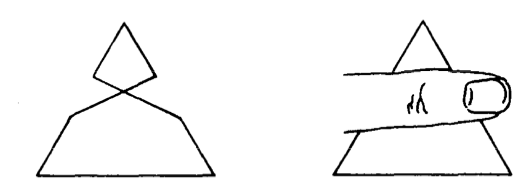
\includegraphics[scale=0.3]{img/kellman_1983_fig2.neg.png}
\end{center}
\emph{source}: Michotte et al (1964) via Kellman and Spelke (1983, figure 2)
 
 
 
\section{Knowledge of Objects: Conclusions}
 
 
 
\section{Core Knowledge}
 
For someone to have \textit{core knowledge of a particular principle or fact} is for her to have a core system where 
either the core system includes a representation of that principle or else the principle plays a special role in describing the core system.
 
\subsection{Two-part definition}
 
‘Just as humans are endowed with multiple, specialized perceptual systems, so we are endowed with multiple systems for representing and reasoning about entities of different kinds.’
\citep[p.\ 517]{Carey:1996hl}
 
‘core systems are 
largely innate 
encapsulated 
unchanging 
arising from phylogenetically old systems 
built upon the output of innate perceptual analyzers’ 
\citep[p.\ 520]{Carey:1996hl}.
 
\textit{Note} There are other, slightly different statements \citep[e.g.][]{carey:2009_origin}.
 
\subsection{Compare modularity}
 
Modules are ‘the psychological systems whose operations present the world to thought’; 
they ‘constitute a natural kind’; and 
there is ‘a cluster of properties that they have in common’ \citep[p.\ 101]{Fodor:1983dg}.
 
These properties include:
 
\begin{itemize}
 
\item domain specificity (modules deal with ‘eccentric’ bodies of knowledge)
 
\item limited accessibility (representations in modules are not usually inferentially integrated with knowledge)
 
\item information encapsulation (modules are unaffected by general knowledge or representations in other modules)
 
\item innateness (roughly, the information and operations of a module not straightforwardly consequences of learning; but see \citet{Samuels:2004ho}).
 
\end{itemize}
 
\subsection{Objection}
 
‘there is a paucity of … data to suggest that they are the only or the best way of carving up the processing,
 
‘and it seems doubtful that the often long lists of correlated attributes should come as a package’
\citep[p.\ 759]{adolphs_conceptual_2010}
 
‘we wonder whether the dichotomous characteristics used to define the two-system models are … perfectly correlated …
[and] whether a hybrid system that combines characteristics from both systems could not be … viable’
\citep[p.\ 537]{keren_two_2009}
 
‘the process architecture of social cognition is still very much in need of a detailed theory’
\citep[p.\ 759]{adolphs_conceptual_2010}
\citep[p.\ 517]{Carey:1996hl}
 

%--- end paste
%--------------- 
 
\footnotesize 
\bibliography{$HOME/endnote/phd_biblio}

\end{multicols}

\end{document}